\documentclass[12pt]{article}

\usepackage{styles/sbc-template}
\usepackage{graphicx,url}
\usepackage[utf8]{inputenc}
\usepackage[american]{babel}
% two images, same frame, side by side
\usepackage{subfig}
\usepackage{booktabs}
\usepackage{soul}
\usepackage{xcolor}
\usepackage{mdframed}

\sloppy

\title{Exploring Energy Flow Classifier to Identify \\ Fraudulent Cryptocurrency Transactions}

\author{anonymous}
\address{anonymous}
% \author{Kevin S. Araujo\inst{1}, Rodrigo Bonifacio de Almeida\inst{1}, 
%   Fabiano Cavalcanti Fernandes\inst{2} }


% \address{Departamento de Ciências da Computação -- Universidade de Brasília (UnB) \\
%   -- Campus Universitário Darcy Ribeiro, Brasília-DF
% \nextinstitute
%   Instituto Federal de Brasília (IFB) -- Taguating, DF -- Brazil
%   \email{kevin.araujo@aluno.unb.br, rbonifacio@unb.br, fabiano.fernandes@ifb.edu.br}
% }

\begin{document} 

\maketitle

\begin{abstract}
  This is a work in progress.
\end{abstract}

\section{Introduction} \label{sec:introduction}
Bitcoin is an electronic transaction system operating without a third-party moderator~\cite{nakamoto2008bitcoin}. It is built
upon blockchain technology, where an immutable ledger of financial transactions is maintained through mathematics, programming,
and advanced cryptography. This distributed ledger architecture eliminates the need for central authorities to establish trust.
Although Bitcoin was designed to circumvent vulnerabilities in the traditional financial system \cite{nakamoto2008bitcoin},
it is not immune to manipulation and anomalous activities, necessitating robust detection mechanisms~\cite{fang2022cryptocurrency,
zhang2020financial,zainal2018review}. 

Indeed, cryptocurrency-related fraud has emerged as a significant threat, causing substantial financial losses and shaking
trust in the digital asset ecosystem. In 2023, for instance, illicit addresses received \$24.2 billion in cryptocurrency,
indicating the scale of financial losses from scams, stolen funds, and other illicit activities \cite{chainalysis2024cryptocrime}.
These activities not only cause direct monetary damage to individuals and institutions but also have broader implications,
such as undermining the legitimacy of cryptocurrency markets and hindering the widespread adoption of blockchain technology.
The need to develop effective methods for detecting and preventing cryptocurrency fraud is crucial to protect participants,
maintain market integrity, and ensure the sustainable growth of the cryptocurrency industry \cite{scharfman2024, Khiari2025}.

However, detecting anomalous patterns within the intricate data streams of cryptocurrency transactions poses a significant
challenge. Like many modern datasets, these transactions are characterized by high dimensionality, evolving characteristics,
and a substantial volume, which complicates the application of traditional anomaly detection methods. In this context, the
Energy-based Flow Classifier (EFC) presents a promising approach rooted in statistical physics. Originally formulated using
the Inverse Potts model \cite{pontes2019}, the EFC characterizes the probability distribution of normal data flows through
an energy function derived from observed data patterns \cite{pontes2019}. Previous research has demonstrated the utility
of EFC in classifying unusual network traffic, suggesting its potential for adapting to detect fraudulent activity within
cryptocurrency systems \cite{pontes2019, souza2022novelopensetenergybased}.

Building upon the promise of the Energy-based Flow Classifier (EFC) framework, this paper presents a comprehensive empirical
evaluation of its application to detecting illicit Bitcoin transactions. To this end, we first replicate a previous study
that employs machine learning algorithms such as K-Nearest Neighbors, One-Class Support Vector Machine, and Isolation Forest
for anomaly detection on the Elliptic dataset \footnote{Available at https://www.kaggle.com/ellipticco/elliptic-data-set}.
We then investigate the use of EFC as a potential alternative to these machine learning approaches, using the same dataset
for consistency. Our findings confirm the EFC's ability to distinguish between licit and illicit transaction patterns based
on their energy profiles, showing strong performance in identifying illegal activity even when trained solely on licit data.
However, the results also highlight the critical sensitivity to specific configuration parameters. In particular, we observe
significant trade-offs between maximizing the detection rate of illicit transactions (recall) and minimizing false positives
(precision), especially concerning the energy threshold that defines anomalous behavior. Addressing the significant challenge
of label scarcity inherent in datasets like Elliptic is crucial for developing effective fraud detection systems.
Traditional supervised machine learning methods often struggle in such scenarios due to the limited availability of
labeled illicit examples. This motivates the exploration of alternative approaches, particularly those capable of learning
from predominantly normal data. The Energy-based Flow Classifier (EFC) emerges as a promising candidate in this regard.
Originally proposed for network intrusion detection \cite{pontes2019, souza2022novelopensetenergybased}, EFC was designed
specifically to address key limitations of conventional ML classifiers, including the reliance on extensive labeled datasets.
A core strength highlighted in its foundational work is its ability to function as an anomaly-based classifier, inferring
a statistical model of normal behavior using only labeled *benign* (or licit, in our context) examples
\cite{souza2022novelopensetenergybased}. Deviations from this learned norm, characterized by higher 'energy' scores, are
then flagged as potential anomalies. This one-class learning paradigm directly tackles the label scarcity issue prevalent
in the Elliptic dataset, allowing us to model legitimate transaction patterns effectively even with few confirmed illicit
instances. Furthermore, EFC's demonstrated adaptability across different data distributions in network traffic analysis
suggests potential robustness in the dynamic environment of cryptocurrency transactions. Consequently, this paper evaluates
the suitability and performance of EFC for identifying illicit Bitcoin transactions by leveraging its capacity to model
normality from available licit data.

In summary, the main contributions of this paper are:

\begin{itemize}
    \item Novel Application and Empirical Evaluation of EFC for One-Class Bitcoin Anomaly Detection;
    \item In-depth analysis of the impact of data balancing and feature selection techniques on EFC's efficacy for
    identifying illicit transactions;
    \item Demonstration of a combined feature selection and data balancing (SMOTE) strategy as a robust approach for enhancing
    EFC performance on imbalanced cryptocurrency datasets.
\end{itemize}

\section{Background and Related Work} \label{sec:background}
Financial market manipulation, traditionally associated with actions taken by state-level entities often concerning currency
exchange rates \cite{domanski2011currency, market_manipulation_detection_2022}, takes on a different character in the realm
of cryptocurrencies. Cryptocurrency manipulation typically involves deceptive strategies employed by individuals or coordinated
groups aiming to artificially distort market prices or activity, usually for illicit profit \cite{cryptocurrency_arket_manipulation_2021}.
Understanding these tactics is crucial for developing effective detection mechanisms.

Among the prevalent forms of cryptocurrency fraud are pump-and-dump schemes and wash trading. \textbf{Pump-and-dump fraud}
involves orchestrating an artificial inflation of a cryptocurrency's price ("pump") through misleading promotions or coordinated
buying, attracting unsuspecting investors. The manipulators then sell their holdings ("dump") at the peak price, causing
a market crash and significant losses for later investors \cite{karim2018manipulation}. \textbf{Wash trading}, conversely,
creates a false impression of high trading volume and liquidity. This is achieved when an entity or colluding group
simultaneously buys and sells the same asset, often using multiple accounts or automated bots, effectively trading with
themselves. The goal is to make the asset appear more active and desirable than it is, thereby manipulating market sentiment
and potentially influencing its price \cite{gandal2018price, edelman2018detecting}. The decentralized and pseudonymous
nature of many cryptocurrency platforms can exacerbate the challenges in detecting and preventing such manipulations.

Addressing the challenge of identifying anomalous patterns within complex data streams, such as financial transactions,
requires robust methodologies. One promising approach, grounded in statistical physics, is the \textbf{Energy-based Flow Classifier (EFC)}.
Originally proposed using the Inverse Potts model to analyze network traffic data \cite{pontes2019}, EFC operates on the
principle of assigning an "energy" score to data points or flows. The model is trained to learn the probability distribution
of normal system behavior, associating typical, expected patterns (e.g., legitimate transactions) with low-energy states.
Conversely, configurations that deviate significantly from this learned normality, potentially representing anomalies or
malicious activities, manifest as high-energy states. This energy score provides a quantitative measure of typicality.
Subsequent research has extended the EFC framework, demonstrating its utility in classifying unusual network traffic for
intrusion detection and highlighting its potential for open-set recognition—identifying novel anomalies not seen during
training \cite{pontes2019, souza2022novelopensetenergybased}.

The EFC framework appears particularly well-suited for detecting anomalous Bitcoin transactions for several key reasons.
Firstly, its fundamental design as an anomaly detector allows it to learn the characteristics of *normal* (Licit) behavior,
often from unlabeled or predominantly normal data. It then identifies anomalies (potentially Illicit transactions) as
deviations exhibiting high 'energy' relative to this learned norm. This inherent capability to operate in a one-class or
unsupervised manner directly addresses the significant challenge of label scarcity common in financial fraud datasets like
Elliptic \cite{bansal2022systematic}. Secondly, the energy function provides a holistic measure derived from
the interplay of multiple features, potentially capturing complex, subtle deviations in the high-dimensional feature space
of Bitcoin transactions that simpler methods might miss \cite{wilson2024future}. Given its prior success in
analogous domains involving complex flow data \cite{pontes2019, souza2022novelopensetenergybased}, we hypothesize that
EFC's unique characteristics offer advantages for identifying illicit activities within the Bitcoin blockchain.

Detecting illicit transactions in cryptocurrencies is fundamentally an anomaly detection task. Various approaches have been 
explored, ranging from rule-based systems identifying known patterns to sophisticated machine learning techniques
\cite{samariya2023comprehensive, li2023survey}.
Traditional anomaly detection methods often face challenges when applied to cryptocurrency data due to its high dimensionality,
the dynamic and evolving nature of transaction patterns, significant class imbalance (illicit transactions being rare), and
the sheer volume of data \cite{pallathadka2022cryptocurrency}. Techniques like statistical process control, clustering-based
methods (e.g., DBSCAN, k-means variations), and distance-based methods (e.g., k-Nearest Neighbors anomaly detection)
have been applied, each with varying degrees of success and limitations, particularly concerning scalability and the ability
to capture complex, non-linear relationships \cite{hilal2022financial}.

Building on these general principles, numerous machine learning models have been specifically investigated for identifying
fraud and money laundering within the Bitcoin ecosystem. Supervised learning approaches, such as Random Forests, Support
Vector Machines (SVM), Multilayer Perceptrons (MLP), and Gradient Boosting Machines, have shown promise when sufficient
labeled data is available \cite{lorenz2021machinelearningmethodsdetect, chen2021bitcoin}. However, their performance heavily
relies on the quality and quantity of labeled examples, which is often a bottleneck. Consequently, semi-supervised and
unsupervised methods, including One-Class SVM (OC-SVM) and Isolation Forests, have gained attention as they can leverage
unlabeled data or focus solely on modeling normal behavior \cite{lorenz2021machinelearningmethodsdetect, kehinde2024machine}.
More recently, Graph Neural Networks (GNNs) have emerged as a powerful tool, explicitly leveraging the graph structure of
the blockchain to capture relational information between transactions, which can be crucial for identifying complex illicit
schemes \cite{weber2019antimoneylaunderingbitcoinexperimenting}. Our work contributes to this landscape by evaluating
EFC, an alternative physics-inspired one-class approach, assessing its performance against the backdrop of these established
techniques, particularly focusing on its behavior under label scarcity.

\section{Study Settings} \label{sec:methods}
This section details the data and methods employed in our study, which builds upon the foundational research presented
by \cite{lorenz2021machinelearningmethodsdetect}. That work explored the use of various machine learning classifiers
(e.g., Random Forest, SVM, MLP) applied to engineered features from the Elliptic dataset to identify illicit Bitcoin transactions,
specifically tackling the inherent challenge of label scarcity. While demonstrating the potential of standard ML techniques,
their approach relied on supervised or semi-supervised frameworks requiring at least some labels. Our research
diverges by investigating the Energy Flow Classifier (EFC). 

\subsection{Dataset Description} \label{subsec:dataset}
This study utilizes the Elliptic dataset, a publicly available graph dataset of Bitcoin transactions introduced by 
\cite{weber2019antimoneylaunderingbitcoinexperimenting} and subsequently used in foundational studies on machine
learning for Bitcoin money laundering detection, including the work by~\cite{lorenz2021machinelearningmethodsdetect}
which highlighted the challenges of label scarcity. The dataset represents a temporal subgraph of the public Bitcoin
blockchain, focusing on transactions involving entities identified by Elliptic Ltd., a company specializing in blockchain
analytics and financial crime prevention. It captures transaction patterns over 49 distinct time steps, where each step
corresponds roughly to a two-week period. The full dataset comprises 203,769 transaction nodes and 234,355 directed edges
representing the flow of Bitcoin between transactions.

Each transaction (node) in the graph is described by a set of 166 anonymized features. One feature explicitly denotes the
time step (1 to 49). The remaining 165 features are local transactional properties, including aggregated information about
the transaction's inputs and outputs (e.g., number, amounts, fees) and potentially aggregated statistics from its immediate
neighborhood in the transaction graph. These features are provided in a normalized or standardized form, obscuring raw
values but preserving relational patterns crucial for machine learning analysis. The graph structure itself, defined by
the edges connecting transactions where the output of one becomes the input of another, provides contextual information
about the flow of funds---although our EFC implementation primarily focuses on the
node features. A key characteristic of the Elliptic dataset is its label scarcity---while the entire dataset contains over
200,000 transactions, only a subset of 46,564 transactions is explicitly labeled. This represents a central challenge addressed by 
\cite{lorenz2021machinelearningmethodsdetect} and serves as a motivation for exploring EFC in this domain.  
The labels classify transactions into two main categories:

\begin{description}
    \item [Licit Transactions:] Transactions associated with known legitimate entities such as exchanges, miners, wallet providers,
      and other regulated services (42,019 instances in the original labeled set).
    \item [Illicit Transaction:] Transactions linked to known illicit activities, including scams, ransomware, terrorist financing,
      Ponzi schemes, and dark market operations (4,545 instances in the original labeled set).
\end{description}

\begin{table}[htbp]
  \centering
  \caption{Summary Statistics of the Elliptic Dataset (based on \cite{weber2019antimoneylaunderingbitcoinexperimenting}).}
  \label{tab:dataset_summary}
  \begin{small}
  \begin{tabular}{lr}\toprule
    Characteristic        & Value \\ \midrule
    Total of Transactions (Nodes) & 203,769 \\
    Total of Edges           & 234,355 \\
    Time Steps            & 49 \\
    Features per Node     & 166 \\
    Labeled Transactions  & 46,564 (\textasciitilde23\%) \\
    \quad - Licit         & 42,019 (\textasciitilde90.2\% of labeled) \\
    \quad - Illicit       & 4,545 (\textasciitilde9.8\% of labeled) \\
    Unlabeled Transactions & 157,205 (\textasciitilde77\%) \\ \bottomrule
  \end{tabular}
  \end{small}
\end{table}

\subsection{Data Preprocessing} \label{subsec:preprocessing}
Preparing the Elliptic dataset for EFC involved several key steps focused on handling labels, selecting relevant features,
scaling the data appropriately, and partitioning it for training and evaluation in a temporally meaningful way.

To prepare the dataset (Section~\ref{subsec:dataset}), we filtered transactions based on their assigned labels. Since the
EFC model learns patterns from \textit{normal} data to detect anomalies, transactions labeled as \textit{Licit} were used
as the normal class for training. In contrast, transactions labeled as \textit{Illicit} were treated as anomalies and reserved
for evaluation. Transactions with \textit{Unknown} labels were excluded from both training and testing to ensure that the
evaluation relied solely on transactions with a known ground truth. For the binary classification task (\textit{licit} vs.
\textit{illicit}), labels were mapped to numerical values—0 for licit and 1 for illicit.

Second, we performed feature selection and transformation. Of the 166 features available for each transaction, the feature
explicitly indicating the time step (ranging from 1 to 49) was removed. While this temporal information was essential for
partitioning the data, it was excluded from the EFC model's input, as the model focuses on intrinsic transaction properties
rather than absolute temporal position. The remaining 165 anonymized features---representing transactional and local graph
characteristics---were retained as inputs to the EFC. Although the original dataset description reports some form of
normalization~\cite{weber2019antimoneylaunderingbitcoinexperimenting}, we decided to apply the Min-Max scaling to the
[0, 1] range to ensure consistency and enhance the stability of energy calculations within the EFC framework. Scaling was
applied separately to the training and test sets, with the scaler fitted exclusively on the training data to prevent data leakage.

Third, we implemented a temporal data split, in line with common practice for this dataset 
\cite{weber2019antimoneylaunderingbitcoinexperimenting, lorenz2021machinelearningmethodsdetect}, to simulate a realistic
scenario in which a model trained on historical data is used to detect fraudulent activity in future transactions.
Transactions from time steps 1 to 34 were allocated to the training set, while those from time steps 35 to 49 were reserved
for testing. The EFC model was trained exclusively on licit (normal) transactions from the training period (time steps 1-34).
The test set (time steps 35-49) included both licit and illicit transactions, enabling an evaluation of the model's ability
to assign higher energy scores to previously unseen illicit transactions compared to unseen licit ones.

\subsection{Energy Flow Classifier Configuration} \label{subsec:efc_implementation}

For detecting illicit transactions within the Elliptic dataset, we employed the Energy Flow Classifier (EFC), leveraging
the Python package implementation \cite{efc_package_github} based on the recommendations by Pontes et al.
\cite{pontes2019,souza2022novelopensetenergybased}. EFC operates on the premise that normal system behavior corresponds
to low-energy states, while anomalies or deviations manifest as high-energy states. Our implementation specifically
utilizes EFC as a one-class anomaly detector, tailored to the label scarcity challenge inherent in the dataset.

To set up EFC in our experiment, we extended the class-based interface provided by the EFC Python package, specifically
by overriding the \texttt{EnergyBasedFlowClassifier} class to tailor its behavior to our evaluation needs. In our implementation,
we configured three key EFC hyperparameters: \texttt{n\_bins}, \texttt{cutoff\_quantile}, and \texttt{pseudocounts}.
The \texttt{n\_bins} parameter controls the discretization of input features, dividing each feature's range into a specified
number of bins. These bins form the basis for estimating state probabilities and computing energy values. Based on preliminary
experiments~\cite{reproducibility}, we used \texttt{n\_bins = 30}. The \texttt{cutoff\_quantile} parameter sets the anomaly
threshold by determining the energy value corresponding to a quantile of the training data's energy distribution. For instance,
a setting of \texttt{cutoff\_quantile = 0.90} classifies any sample with an energy score above the 90th percentile as anomalous.
Finally, \texttt{pseudocounts} addresses the issue of zero probabilities when encountering states not seen in the training
data. We used a small \texttt{pseudocounts} of \texttt{0.10} to ensure numerical stability during energy computation.

Regarding the \emph{training process}, a central aspect of our EFC configuration is its alignment with the anomaly detection
setting under label scarcity. As outlined in Section~\ref{subsec:preprocessing}, the EFC model was trained exclusively on
licit (normal) transactions from the training period (time steps 1--34) by invoking its \texttt{fit} method. This follows
the one-class classification paradigm, in which the model learns the energy landscape associated with legitimate Bitcoin
transactions based solely on verified normal examples. Illicit transactions were entirely excluded from the training phase
to preserve the model's ability to generalize and detect anomalies without prior exposure to them.

During the evaluation phase, the trained EFC model's \texttt{predict} method was applied to the test set---transactions
from time steps 35--49, which contained both licit and illicit instances. For each test transaction, the EFC computed an
energy score based on its features and the probability distributions learned during training. If a transaction's energy
score exceeded the pre-determined cutoff threshold (derived from the \texttt{cutoff\_quantile} applied to the training data's
energy distribution), it was classified as anomalous (predicted illicit); otherwise, it was classified as normal (predicted licit).
The energy scores were also used to compute evaluation metrics such as AUC, which assess ranking performance rather than
relying on a fixed classification threshold.

\section{Goal, Questions, and Metrics} \label{subsec:task}
The primary goal of this study is to evaluate the effectiveness of the Energy Flow Classifier (EFC), configured
as described in Section \ref{subsec:efc_implementation}, for identifying illicit transactions within the Elliptic
Bitcoin dataset. This aligns with the broader goal of exploring alternative methodologies, particularly those suited for
label scarcity, compared to the supervised approaches examined by \cite{lorenz2021machinelearningmethodsdetect}. Our aim
is to answer the following research question: \emph{How effective is the Energy-Based Flow Classifier (EFC) under conditions
of label scarcity in identifying illicit transactions in the Elliptic Bitcoin dataset?}

Specifically, our research is thus framed as a \emph{one-class anomaly detection problem}. Having trained the EFC model exclusively
on Licit transactions from the initial time steps (1-34), the objective is to assess its ability to distinguish between
licit and illicit transactions in the subsequent, unseen time steps (35-49) of the test set. This evaluation involves
two main perspectives:

\begin{enumerate}
    \item \textbf{Classification Performance:} Using the energy threshold derived from the training data, based on the
      \texttt{cutoff\_quantile}, we assess how well EFC classifies unseen transactions as either licit (below threshold)
      or illicit (above threshold). Performance is measured using standard classification metrics suitable for imbalanced
      datasets, such as Precision, Recall, F1-Score, and potentially Balanced Accuracy, calculated on the labeled test set.
      
    \item \textbf{Ranking Performance:} Independent of a specific threshold, we evaluate EFC's ability to assign consistently
      higher energy scores to illicit transactions compared to licit transactions in the test set. This is primarily
      assessed using the Area Under the Receiver Operating Characteristic Curve (AUC-ROC), which measures the model's
      ability to rank anomalies higher than normal instances across all possible thresholds.
\end{enumerate}

The outcomes of this research provide insights into the potential of the EFC model as a viable tool for detecting fraudulent or
anomalous Bitcoin transactions. By leveraging its unsupervised, energy-based approach, EFC aims to address challenges such
as label scarcity and to identify novel deviations from normal transaction behavior. 

Model performance was assessed using a combination of quantitative metrics and visual analysis. We use the \textbf{F1-Score Macro Average}
as the primary evaluation metric, following the same design decision of \cite{lorenz2021machinelearningmethodsdetect}.
This metric calculates the F1-score for each class (Licit and Illicit) independently and then averages them, providing a
balanced measure of performance across both classes, which is crucial given the inherent class imbalance. 

We also leverage \textbf{Specific Metrics for the Illicit Class}, since our primary interest lies in detecting anomalous
transactions. As such, we also report Precision, Recall, and the F1-Score specifically calculated for the Illicit class
based on the classification derived from the \texttt{cutoff\_quantile} threshold. These metrics offer direct insight into
the model's effectiveness in identifying illicit transactions and the associated trade-offs (e.g., false positives vs. false negatives). 

Finally, we highlight the \textbf{EFC Energy Distributions.} For each experiment we detail in the next section, we show
histograms comparing the distribution of EFC energy scores assigned to Licit versus Illicit transactions in the test set
that were generated. These plots provide a visual assessment of the model's separation capability.

\section{Results} \label{sec:results}

This section presents the empirical findings from the application of the Energy Flow Classifier (EFC) to the task of
identifying illicit transactions within the Elliptic Bitcoin dataset. Following the methodology outlined in Section
\ref{sec:methods}, the EFC was employed primarily as a one-class anomaly detector, trained exclusively on transactions
labeled as Licit from the initial time steps (1-34). The core objective was to evaluate the model's capability to distinguish
these known Licit patterns from potentially anomalous Illicit transactions present in the unseen test set (time steps 35-49).
Performance is assessed based on the EFC's ability to assign distinct energy scores to the two classes and evaluated using
metrics appropriate for imbalanced anomaly detection scenarios. The subsequent subsections detail the outcomes of specific
experiments conducted, focusing on the model's baseline performance and sensitivity to key configuration parameters under
the defined experimental setup. We performed three primary
experiments focusing on data balancing, feature engineering/selection, and model comparison/tuning, respectively. All experiments
utilized the Elliptical dataset, preprocessed as described previously, employing a standard train-test split methodology.

              
%\subsection{Shared Experimental Setup} \label{subsec:shared_setup}
% Unless explicitly stated otherwise in the description of a specific experiment, the following setup, derived from the procedures
% detailed in Section \ref{sec:methods}, was consistently used across the results presented below:

% \begin{itemize}
%     \item \textbf{Dataset Split:} The EFC model was trained exclusively on transactions labeled as Licit from time steps
%       1 to 34. Evaluation was performed on the test set containing both Licit and Illicit transactions from time steps
%       35 to 49. Transactions labeled 'Unknown' were excluded from both training and testing.
%     \item \textbf{Feature Set:} The input to the EFC model consisted of the 165 anonymized features described in Section
%       \ref{subsec:dataset}, after removing the time step feature. These features were scaled to the range [0, 1] using
%       Min-Max scaling, with the scaler fitted only on the training data (Licit transactions, steps 1-34).
%     \item \textbf{EFC Configuration:} The core EFC implementation (Section \ref{subsec:efc_implementation}) utilized the
%       following default hyperparameters based on initial tuning and common practice:
%         \begin{itemize}
%             \item Number of bins for feature discretization \texttt{n\_bins=30}
%             \item Cutoff quantile for anomaly threshold \texttt{cutoff\_quantile=0.9} (meaning the energy threshold is set at
%               the 90th percentile of the energy distribution of the Licit training data)
%             \item Pseudocounts \texttt{pseudocounts=0.1} (to handle zero probabilities)
%         \end{itemize}
%         \item \textbf{Evaluation Metrics \& Outputs:} Model performance was assessed using a combination of quantitative
%           metrics and qualitative analysis:
%           \begin{itemize}
%               \item \textbf{F1-Score (Macro Average):} As the primary evaluation metric, we adopted the macro-averaged F1-score,
%                 consistent with the benchmark study by \cite{lorenz2021machinelearningmethodsdetect}. This metric calculates the
%                 F1-score for each class (Licit and Illicit) independently and then averages them, providing a balanced measure
%                 of performance across both classes, which is crucial given the inherent class imbalance.
%               \item \textbf{Class-Specific Metrics (Illicit Class):} While F1-Macro provides an overall view, our primary
%                 interest lies in detecting the Illicit class (class 1). Therefore, we also report Precision, Recall, and
%                 the F1-Score specifically calculated for the Illicit class based on the classification derived from the
%                 \texttt{cutoff\_quantile} threshold. These metrics offer direct insight into the model's effectiveness in
%                 identifying illicit transactions and the associated trade-offs (e.g., false positives vs. false negatives).
%               \item \textbf{EFC Energy Distributions:} For each experiment, histograms comparing the distribution of EFC
%                 energy scores assigned to Licit versus Illicit transactions in the test set were generated. These plots
%                   provide a visual assessment of the model's separation capability.
%               \item \textbf{Detailed Results Storage:} Key information for each experimental run, including the sizes of
%                 the training and testing datasets (and their class distributions), the calculated performance metrics,
%                 and the confusion matrix, were systematically collected and saved into individual CSV files for detailed
%                 comparison and analysis across experiments.
%           \end{itemize}
% \end{itemize}

% The following subsections will now present the results from the specific experiments conducted under this framework, highlighting
% deviations from this shared setup where applicable.

%\subsection{Experiments} \label{subsec:experiments}

%This section details the experimental evaluations conducted to assess the proposed methodologies. 
% We performed three primary
% experiments focusing on data balancing, feature engineering/selection, and model comparison/tuning, respectively. All
% experiments utilized the EFC dataset, preprocessed as described previously, employing a standard train-test split methodology.

\subsection{Experiment 1: Impact of Data Balancing Techniques} \label{subsec:experiment_1}

This experiment examined the impact of different data balancing strategies on classification performance using the inherently
imbalanced EFC dataset.

Baseline performance was measured using the original, unbalanced dataset. This baseline was then compared against four widely
adopted balancing techniques, each applied to both the training and test datasets: (a) creating a balanced subset by undersampling
the majority class prior to the train-test split, (b) applying the Synthetic Minority Over-sampling Technique (SMOTE), (c)
performing random oversampling of the minority class, and (d) performing random undersampling of the majority class. To
ensure a fair comparison, the composition of the test set was kept consistent across most techniques.

Model performance was evaluated using Accuracy, Precision, Recall, weighted F1-Score, Macro F1-Score, and confusion matrices.
Table~\ref{tab:efc_consolidated_results} presents a summary of the dataset characteristics resulting from each balancing
strategy, along with the corresponding classification outcomes.


\begin{table}[htbp]
  \centering
  \caption{EFC Performance Across Data Balancing Techniques (Experiment 1).}
  \label{tab:balancing_results}
  \resizebox{\textwidth}{!}{
    \begin{tabular}{lrrrrrrrrr}
      \toprule
      \textbf{Configuration} & \textbf{TP} & \textbf{FN} & \textbf{FP} & \textbf{TN} & \textbf{Accuracy} & \textbf{Precision}
      & \textbf{Recall} & \textbf{F1-Score} & \textbf{F1-Macro} \\
      & & & & & & & & \textbf{(Weighted)} & \\
      \midrule
      Unbalanced Dataset (Baseline)$^{a}$ & 15117 & 470 & 1064 & 19 & 0.908 & 0.876 & 0.908 & 0.891 & 0.488 \\
      Balanced Dataset (Equally Dist.)$^{b}$ & 516 & 848 & 37 & 1326 & 0.675 & 0.772 & 0.675 & 0.644 & 0.644 \\
      SMOTE$^{b}$ & 10831 & 1775 & 530 & 12076 & 0.909 & 0.913 & 0.909 & 0.908 & \textbf{0.908} \\
      Random Oversampling$^{a}$ & 15393 & 194 & 1013 & 70 & 0.928 & 0.895 & 0.928 & 0.907 & 0.533 \\
      Random Undersampling$^{a}$ & 13791 & 1796 & 412 & 671 & 0.868 & 0.926 & 0.868 & 0.890 & 0.652 \\
      \bottomrule
    \end{tabular}
  }
  \par\medskip
  \footnotesize
  \textit{Note: TP=True Positives, FN=False Negatives, FP=False Positives, TN=True Negatives. Metrics are rounded. F1-Score
    is weighted average. F1-Macro for SMOTE is bolded as it's the highest among these techniques. Test set composition:
    ($^{a}$) Imbalanced, ($^{b}$) Balanced.}
\end{table}

\begin{figure}[!tph]
  \centering
  \subfloat[Unbalanced Dataset.]{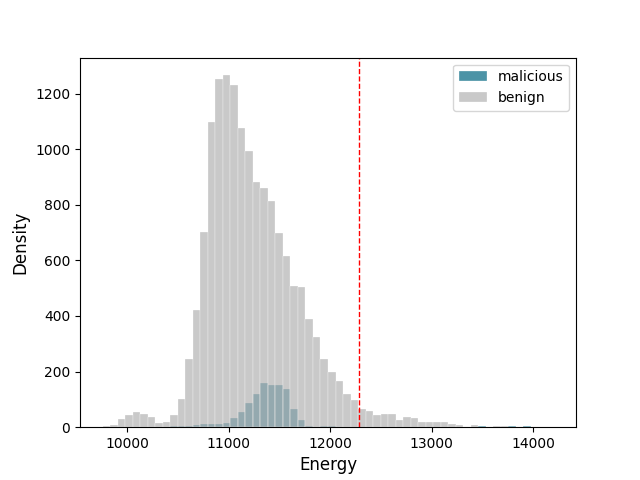
\includegraphics[width=0.35\textwidth]{figures/experiment-1/1_unbalanced_dataset.png}\label{fig1:1_unbalanced_dataset}}
  \subfloat[Balanced Dataset.]{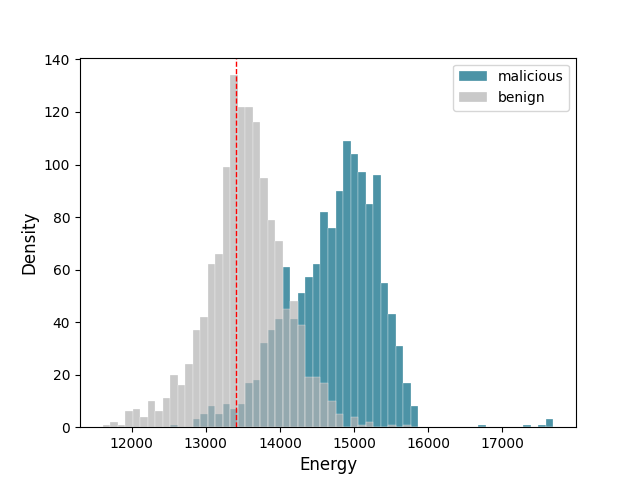
\includegraphics[width=0.35\textwidth]{figures/experiment-1/2_balaced_dataset.png}\label{fig2:2_balaced_dataset}}
  \subfloat[SMOTE.]{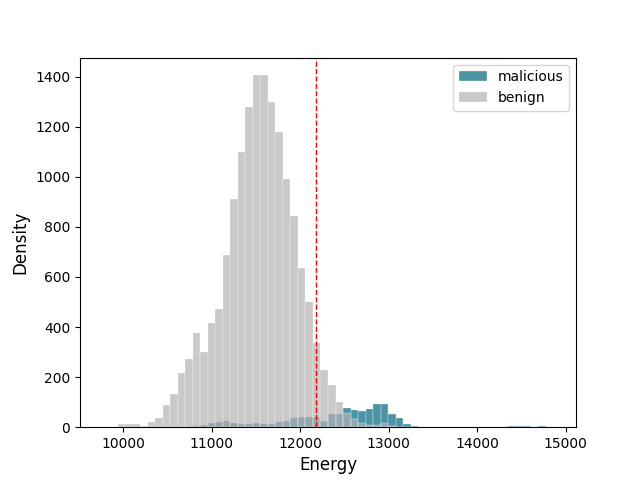
\includegraphics[width=0.35\textwidth]{figures/experiment-1/3_smote_minority_full_test_dataset.png}\label{fig3:3_smote_minority}}
  \caption{Experiment 1: Energy Distribution of Licit and Illicit Transactions.}
\end{figure}

% \paragraph{Discussion of Experiment 1 Results}
The results from Experiment 1 (Table~\ref{tab:balancing_results}) clearly illustrate the EFC's sensitivity to class imbalance
and the significant impact of balancing techniques. The baseline ``Unbalanced Dataset,'' when tested on an imbalanced test
set, yielded a low F1-Macro score of 0.488, confirming the difficulty in detecting the minority illicit class without
intervention. This result is most likely due to the nature of one-class classifiers and imbalanced data. Applying SMOTE
and evaluating on a balanced test set resulted in a striking improvement, with an F1-Macro of 0.908. This suggests that
EFC can perform exceptionally well if the training data is appropriately balanced and the evaluation scenario also reflects
a more balanced class distribution. 

Other techniques applied to the training data but evaluated on an imbalanced test set
also showed improvements over the baseline: Random Oversampling achieved an F1-Macro of 0.533, and Random Undersampling
reached 0.652. This indicates that even simpler balancing methods can enhance EFC's performance on imbalanced test data,
with undersampling being more effective than oversampling in this specific setup. The ``Balanced Dataset (Equally Dist.)''
technique, which involved undersampling the majority class to create a balanced training and test set, achieved an F1-Macro
of 0.644. While better than the baseline, it did not match SMOTE's performance on a balanced test set, suggesting that
SMOTE's approach of generating synthetic minority samples is more beneficial for EFC in such conditions. 

The stark contrast in F1-Macro scores, particularly between SMOTE on a balanced test set and other techniques on imbalanced
test sets, underscores the critical influence of test set composition on this metric.

\subsection{Experiment 2: Impact of Feature Selection} \label{subsec:experiment_2}

Following the analysis of data balancing, our second experiment focused on evaluating the impact of feature selection on
classification performance using the Energy-Based Flow Classifier (EFC). We employed the \texttt{SelectKBest} algorithm
from scikit-learn, utilizing the ANOVA F-value (\texttt{f\_classif}) scoring function to rank and select features based
on their relevance to the class labels. 

In this experiment, we systematically varied the number of selected features ($k$), testing values of $k \in {10, 20, 30,
40, 50, 60}$. We applied the feature selection process to the features and labels of the original unbalanced dataset
\textit{before} the standard train-test split was performed on the resulting reduced feature set. Furthermore, we conducted
two distinct series of runs: one applying feature selection to the complete feature set, including aggregated temporal
features, and another applying it only to the raw node features after explicitly excluding the aggregated ones. This
decision was driven by the need to understand the specific impact and contribution of these aggregated features. 

Aggregated features, which represent statistical summaries of a node's neighborhood (as described in related financial forensics
work, e.g., \cite{weber2019antimoneylaunderingbitcoinexperimenting}), often possess high individual predictive power due
to the condensed information they carry about local graph structure. Including these potentially dominant features in the
\texttt{SelectKBest} process (Scenario 1) could lead to them consistently ranking highest, potentially masking the predictive
contribution of the node's intrinsic, raw features. By running a separate scenario (Scenario 2) where these aggregated
features were removed \textit{before} applying \texttt{SelectKBest}, we aimed to isolate and evaluate the predictive
capability derived solely from the raw node characteristics. This allows for a clearer comparison and a better understanding
of which feature types (raw vs. aggregated) are most crucial for classification, especially when operating under the
dimensionality constraints imposed by selecting only the top $k$ features.

Performance for each value of $k$ and for both feature set scenarios (with and without aggregated features) was assessed
using standard classification metrics (Accuracy, Precision, Recall, F1-Score, and F1-Macro). The objective was to
determine if reducing dimensionality could maintain or improve performance, identify an optimal number of features ($k$),
and understand the contribution of aggregated features within this selection context.
We summarize the results in Table~\ref{tab:fs_excluded_agg_results} Table~\ref{tab:fs_included_agg_results}.

\begin{table*}[htbp]
  \centering
  \caption{EFC Performance with Feature Selection (Aggregated Features Excluded) for Varying k (Experiment 2a).}
  \label{tab:fs_excluded_agg_results}
  \resizebox{\textwidth}{!}{
  \begin{tabular}{lrrrrrrrrr}
    \hline
    \textbf{k Value} & \textbf{TP} & \textbf{FN} & \textbf{FP} & \textbf{TN} & \textbf{Accuracy} & \textbf{Precision} & \textbf{Recall} & \textbf{F1-Score} & \textbf{F1-Macro} \\
    & & & & & & & & \textbf{(Weighted)} & \\
    \hline
    10 & 11317 & 1289 & 598 & 766 & 0.865 & 0.893 & 0.865 & 0.877 & \textbf{0.686} \\
    20 & 11326 & 1280 & 859 & 505 & 0.847 & 0.866 & 0.847 & 0.856 & 0.617 \\
    30 & 11330 & 1276 & 1103 & 261 & 0.830 & 0.839 & 0.830 & 0.834 & 0.542 \\
    40 & 11305 & 1301 & 1341 & 23  & 0.811 & 0.808 & 0.811 & 0.810 & 0.456 \\
    50 & 11291 & 1315 & 1318 & 46  & 0.812 & 0.811 & 0.812 & 0.811 & 0.465 \\
    60 & 11254 & 1352 & 1138 & 226 & 0.822 & 0.833 & 0.822 & 0.827 & 0.527 \\
    \hline
  \end{tabular}
  }
  \par\medskip
  \footnotesize
  \textit{Note: Feature selection excluding aggregated features. TP=True Positives, FN=False Negatives, FP=False Positives,
  TN=True Negatives. Metrics rounded to three decimal places. F1-Score is weighted average. F1-Macro for k=10 is bolded
  as it's the highest.}
\end{table*}

\begin{table*}[htbp]
  \centering
  \caption{EFC Performance with Feature Selection (Aggregated Features Included) for Varying k (Experiment 2b).}
  \label{tab:fs_included_agg_results}
  \resizebox{\textwidth}{!}{
  \begin{tabular}{lrrrrrrrrr}
    \hline
    \textbf{k Value} & \textbf{TP} & \textbf{FN} & \textbf{FP} & \textbf{TN} & \textbf{Accuracy} & \textbf{Precision} & \textbf{Recall} & \textbf{F1-Score} & \textbf{F1-Macro} \\
    & & & & & & & & \textbf{(Weighted)} & \\
    \hline
    10 & 11254 & 1352 & 560 & 804 & 0.863 & 0.896 & 0.863 & 0.876 & \textbf{0.689} \\
    20 & 11297 & 1309 & 656 & 708 & 0.859 & 0.887 & 0.859 & 0.871 & 0.669 \\
    30 & 11309 & 1297 & 789 & 575 & 0.851 & 0.874 & 0.851 & 0.861 & 0.635 \\
    40 & 11296 & 1310 & 991 & 373 & 0.835 & 0.851 & 0.835 & 0.843 & 0.576 \\
    50 & 11291 & 1315 & 1265 & 99  & 0.815 & 0.818 & 0.815 & 0.817 & 0.484 \\
    60 & 11269 & 1337 & 1261 & 103 & 0.814 & 0.819 & 0.814 & 0.816 & 0.485 \\
    \hline
  \end{tabular}
  }
  \par\medskip
  \footnotesize
  \textit{Note: Feature selection including aggregated features. TP=True Positives, FN=False Negatives, FP=False Positives,
  TN=True Negatives. Metrics rounded to three decimal places. F1-Score is weighted average. F1-Macro for k=10 is bolded
  as it's the highest.}
\end{table*}

% \paragraph{Discussion of Experiment 2 Results}
% Experiment 2 investigated the impact of feature selection on EFC's performance, with results presented in
% Table~\ref{tab:fs_excluded_agg_results} (aggregated features excluded) and Table~\ref{tab:fs_included_agg_results}
% (aggregated features included). 

Considering both scenarios, a key observation is that EFC can achieve its best performance with a significantly reduced
feature set. When aggregated features were excluded (Table~\ref{tab:fs_excluded_agg_results}), the highest F1-Macro score
of 0.686 was obtained with only $k=10$ features. Similarly, when aggregated features were included in the selection pool
(Table~\ref{tab:fs_included_agg_results}), the peak F1-Macro was 0.689, also at $k=10$.

This suggests that a small subset of the most relevant features is sufficient for EFC, and including more features beyond
this optimal $k$ (generally $k>20$) tends to degrade performance, likely due to the introduction of noise or less
informative features that can adversely affect EFC's energy calculations. This diminishing return with increasing $k$ is
a common phenomenon in feature selection. The slightly higher F1-Macro obtained when aggregated features were included
(0.689 vs. 0.686) indicates their strong predictive value, even when only a few are selected. These F1-Macro scores represent
an improvement over the baseline (0.488 from Experiment 1) but are not as high as those achieved with data balancing
techniques like Random Undersampling (0.652 on an imbalanced test set) or SMOTE (0.908 on a balanced test set). 

This implies that while feature selection is beneficial for dimensionality reduction and can improve upon the baseline,
addressing class imbalance appears to be a more critical factor for enhancing EFC's F1-Macro score in this dataset. The
results confirm that feature selection can be effective, but might not be a complete solution without tackling imbalance.

% \begin{figure}[!tph]
%   \centering
%   \subfloat[k=10.]{\includegraphics[width=0.3\textwidth]{figures/experiment-2/1-Feature Selection Excluding Aggregate Features,
%   Increasing Value of k={k_size}/Feature Selection Excluding Aggregate Features, Increasing Value of k=10.png}\label{fig4:fs_no_agg_k_10}}
%   \hfill
%   \subfloat[k=20.]{\includegraphics[width=0.3\textwidth]{figures/experiment-2/1-Feature Selection Excluding Aggregate Features,
%   Increasing Value of k={k_size}/Feature Selection Excluding Aggregate Features, Increasing Value of k=20.png}\label{fig5:fs_no_agg_k_20}}
%   \hfill
%   \subfloat[k=30.]{\includegraphics[width=0.3\textwidth]{figures/experiment-2/1-Feature Selection Excluding Aggregate Features,
%   Increasing Value of k={k_size}/Feature Selection Excluding Aggregate Features, Increasing Value of k=30.png}\label{fig6:fs_no_agg_k_30}}
%   \hfill
%   \subfloat[k=40.]{\includegraphics[width=0.3\textwidth]{figures/experiment-2/1-Feature Selection Excluding Aggregate Features,
%   Increasing Value of k={k_size}/Feature Selection Excluding Aggregate Features, Increasing Value of k=40.png}\label{fig7:fs_no_agg_k_40}}
%   \hfill
%   \subfloat[k=50.]{\includegraphics[width=0.3\textwidth]{figures/experiment-2/1-Feature Selection Excluding Aggregate Features,
%   Increasing Value of k={k_size}/Feature Selection Excluding Aggregate Features, Increasing Value of k=50.png}\label{fig8:fs_no_agg_k_50}}
%   \hfill
%   \subfloat[k=60.]{\includegraphics[width=0.3\textwidth]{figures/experiment-2/1-Feature Selection Excluding Aggregate Features,
%   Increasing Value of k={k_size}/Feature Selection Excluding Aggregate Features, Increasing Value of k=60.png}\label{fig9:fs_no_agg_k_60}}
%   \hfill
%   \caption{Experiment 2, Technique A: Feature Selection Excluding Aggregate Features, Increasing Value of k, Energy
%   Distribution Of Licit and Illicit Transactions.}
% \end{figure}

% \begin{figure}[!tph]
%   \centering
%   \subfloat[k=10.]{\includegraphics[width=0.30\textwidth]{figures/experiment-2/2-Feature Selection Excluding Aggregate Features,
%   Increasing Value of k={k_size}/Feature Selection, Increasing Value of k=10.png}\label{fig10:fs_agg_k_10}}
%   \hfill
%   \subfloat[k=20.]{\includegraphics[width=0.30\textwidth]{figures/experiment-2/2-Feature Selection Excluding Aggregate Features,
%   Increasing Value of k={k_size}/Feature Selection, Increasing Value of k=20.png}\label{fig11:fs_agg_k_20}}
%   \hfill
%   \subfloat[k=30.]{\includegraphics[width=0.30\textwidth]{figures/experiment-2/2-Feature Selection Excluding Aggregate Features,
%   Increasing Value of k={k_size}/Feature Selection, Increasing Value of k=30.png}\label{fig12:fs_agg_k_30}}
%   \hfill
%   \subfloat[k=40.]{\includegraphics[width=0.30\textwidth]{figures/experiment-2/2-Feature Selection Excluding Aggregate Features,
%   Increasing Value of k={k_size}/Feature Selection, Increasing Value of k=40.png}\label{fig13:fs_agg_k_40}}
%   \hfill
%   \subfloat[k=50.]{\includegraphics[width=0.30\textwidth]{figures/experiment-2/2-Feature Selection Excluding Aggregate Features,
%   Increasing Value of k={k_size}/Feature Selection, Increasing Value of k=50.png}\label{fig14:fs_agg_k_50}}
%   \hfill
%   \subfloat[k=60.]{\includegraphics[width=0.30\textwidth]{figures/experiment-2/2-Feature Selection Excluding Aggregate Features,
%   Increasing Value of k={k_size}/Feature Selection, Increasing Value of k=60.png}\label{fig15:fs_agg_k_60}}
%   \hfill
%   \caption{Experiment 2, Technique B: Feature Selection Including Aggregate Features, Increasing Value of k, Energy
%   Distribution Of Licit and Illicit Transactions.}
% \end{figure}


\subsection{Experiment 3: Combining Feature Selection and Data Balancing} \label{subsec:experiment_3}

The goal of this third experiment is to investigate the combined impact of feature selection and data balancing on the
performance of the EFC classifier. It builds upon the findings of Experiment~1 (data balancing) and Experiment~2
(feature selection). The central idea is to first reduce the dataset's dimensionality using the feature selection method
identified in Experiment~2, and then apply the SMOTE balancing technique (from Experiment~1) to the reduced training data
before training the EFC model.

In more detail, for each value of $k \in \{10, 20, 30, 40, 50, 60\}$, we applied the \texttt{SelectKBest} algorithm with
the \texttt{f\_classif} scoring function to the original, unbalanced dataset---following the approach used in the first
scenario of Experiment~2---to retain only the top $k$ features. This $k$-feature dataset was then subjected to the SMOTE
procedure. Specifically, we first split the dataset into training and test sets. Next, we applied SMOTE to the training
set to balance the class distribution. The EFC classifier was then trained on this balanced, feature-reduced training data,
and evaluated on the corresponding unbalanced test set (which contained the same $k$ selected features).

We evaluated the performance using standard classification metrics (again, Accuracy, Precision, Recall, F1-Score, and Macro
F1-Score). This evaluation aimed to determine whether applying feature selection before SMOTE could lead to improved classification
performance, compared to using SMOTE on the full feature set (as in Experiment~1) or applying feature selection alone (as in Experiment~2).

We summarize the results in Table~\ref{tab:exp3_smote_fs_results} (Experiment 3a, standard unbalanced test set) and
Table~\ref{tab:exp3_smote_fs_full_test_results} (Experiment 3b, ``Full Test Dataset'' context, also an unbalanced test set). 

In Experiment 3a, the combination yielded a peak F1-Macro score of 0.808 when $k=30$ features were selected before applying
SMOTE. This is a substantial improvement compared to using feature selection alone (Experiment 2, best F1-Macro ~0.689)
and the baseline (0.488). It also surpasses the F1-Macro achieved by Random Undersampling alone (0.652) on a similar imbalanced
test set. That is, combining two effective strategies---dimensionality reduction to focus on salient features and SMOTE to
address imbalance---leads to an improvement on the overall performance. The optimal $k=30$ here is higher than the $k=10$
found in Experiment 2 (FS alone), though, suggesting that SMOTE might benefit from a slightly richer, yet still reduced, feature
set to generate more effective synthetic samples. 

Experiment 3b, conducted under the ``Full Test Dataset'' context (which also utilized an imbalanced test set as per its
note), showed a similar trend, with $k=30$ also yielding the best F1-Macro score of 0.770. While this is still a strong
result and a significant improvement over the baseline and feature selection alone, it is slightly lower than the 0.808
achieved in Experiment 3a. This minor discrepancy, despite both experiments testing on imbalanced sets, could be attributed
to subtle differences in the exact composition or characteristics of the test data partitions used, or slight variations
in the feature subsets selected if the ``Full Test Dataset'' context implied any nuanced differences in the overall feature
pool available before selection for that specific run.

Overall, Experiment 3 shows that a combined strategy of feature selection followed by SMOTE balancing is highly
effective for improving EFC's F1-Macro score on imbalanced test data, outperforming either technique applied in isolation
(when FS is tested on imbalanced data). However, these scores still do not reach the F1-Macro of 0.908 achieved by SMOTE
alone when evaluated on an ideally balanced test set (Experiment 1), further highlighting the profound impact of the
evaluation scenario's balance on the F1-Macro metric.

\begin{table*}[htbp]
  \centering
  \caption{EFC Performance: SMOTE with Feature Selection for Varying k (Experiment 3a).}
  \label{tab:exp3_smote_fs_results}
  \resizebox{\textwidth}{!}{
  \begin{tabular}{lrrrrrrrrr}
    \hline
    \textbf{k Value} & \textbf{TP} & \textbf{FN} & \textbf{FP} & \textbf{TN} & \textbf{Accuracy} & \textbf{Precision} & \textbf{Recall} & \textbf{F1-Score} & \textbf{F1-Macro} \\
    & & & & & & & & \textbf{(Weighted)} & \\
    \hline
    10 & 11319 & 1287 & 369 & 995 & 0.891 & 0.931 & 0.891 & 0.891 & 0.770 \\
    20 & 11326 & 1280 & 263 & 1101 & 0.900 & 0.939 & 0.900 & 0.900 & 0.798 \\
    30 & 11331 & 1275 & 226 & 1138 & 0.903 & 0.942 & 0.903 & 0.903 & \textbf{0.808} \\
    40 & 11272 & 1334 & 223 & 1141 & 0.900 & 0.940 & 0.900 & 0.900 & 0.799 \\
    50 & 11233 & 1373 & 247 & 1117 & 0.894 & 0.935 & 0.894 & 0.894 & 0.780 \\
    60 & 11239 & 1367 & 243 & 1121 & 0.895 & 0.936 & 0.895 & 0.895 & 0.783 \\
    \hline
  \end{tabular}
  }
  \par\medskip
  \footnotesize
  \textit{Note: SMOTE applied to training data after feature selection (including aggregated features). Test set is unbalanced.
  TP=True Positives, FN=False Negatives, FP=False Positives, TN=True Negatives. Metrics rounded. F1-Score is weighted average.
  F1-Macro for k=30 is bolded.}
\end{table*}

\begin{table*}[htbp]
  \centering
  \caption{EFC Performance: SMOTE with Feature Selection (Full Test Dataset Context) for Varying k (Experiment 3b).}
  \label{tab:exp3_smote_fs_full_test_results}
  \resizebox{\textwidth}{!}{
  \begin{tabular}{lrrrrrrrrr}
    \hline
    \textbf{k Value} & \textbf{TP} & \textbf{FN} & \textbf{FP} & \textbf{TN} & \textbf{Accuracy} & \textbf{Precision} & \textbf{Recall} & \textbf{F1-Score} & \textbf{F1-Macro} \\
    & & & & & & & & \textbf{(Weighted)} & \\
    \hline
    10 & 11322 & 1284 & 368 & 996 & 0.882 & 0.894 & 0.882 & 0.917 & 0.739 \\
    20 & 11302 & 1304 & 259 & 1105 & 0.888 & 0.901 & 0.888 & 0.927 & 0.761 \\
    30 & 11313 & 1293 & 218 & 1146 & 0.892 & 0.905 & 0.892 & 0.931 & \textbf{0.770} \\
    40 & 11254 & 1352 & 222 & 1142 & 0.887 & 0.901 & 0.887 & 0.930 & 0.763 \\
    50 & 11258 & 1348 & 249 & 1115 & 0.886 & 0.899 & 0.886 & 0.927 & 0.758 \\
    60 & 11278 & 1328 & 249 & 1115 & 0.887 & 0.901 & 0.887 & 0.927 & 0.760 \\
    \hline
  \end{tabular}
  }
  \par\medskip
  \footnotesize
  \textit{Note: SMOTE applied to training data after feature selection (including aggregated features). Test set is unbalanced
  (1364 Malicious, 12606 Benign). TP=True Positives, FN=False Negatives, FP=False Positives, TN=True Negatives. Metrics rounded.
  F1-Score is weighted average. F1-Macro for k=30 is bolded.}
\end{table*}


\begin{figure}[!tph]
  \centering
  \subfloat[k=10.]{\includegraphics[width=0.30\textwidth]{figures/experiment-3/1-SMOTE With Feature Selection, Increasing
    Value of k={k_size}/SMOTE With Feature Selection, Increasing Value of k=10.png}\label{fig16:fs_smote_k_10}}
  \hfill
  \subfloat[k=20.]{\includegraphics[width=0.30\textwidth]{figures/experiment-3/1-SMOTE With Feature Selection, Increasing
  Value of k={k_size}/SMOTE With Feature Selection, Increasing Value of k=20.png}\label{fig17:fs_smote_k_20}}
  \hfill
  \subfloat[k=30.]{\includegraphics[width=0.30\textwidth]{figures/experiment-3/1-SMOTE With Feature Selection, Increasing
  Value of k={k_size}/SMOTE With Feature Selection, Increasing Value of k=30.png}\label{fig18:fs_smote_k_30}}
  \hfill
  \subfloat[k=40.]{\includegraphics[width=0.30\textwidth]{figures/experiment-3/1-SMOTE With Feature Selection, Increasing
  Value of k={k_size}/SMOTE With Feature Selection, Increasing Value of k=40.png}\label{fig19:fs_smote_k_40}}
  \hfill
  \subfloat[k=50.]{\includegraphics[width=0.30\textwidth]{figures/experiment-3/1-SMOTE With Feature Selection, Increasing
  Value of k={k_size}/SMOTE With Feature Selection, Increasing Value of k=50.png}\label{fig20:fs_smote_k_50}}
  \hfill
  \subfloat[k=60.]{\includegraphics[width=0.30\textwidth]{figures/experiment-3/1-SMOTE With Feature Selection, Increasing
  Value of k={k_size}/SMOTE With Feature Selection, Increasing Value of k=60.png}\label{fig21:fs_smote_k_60}}
  \hfill
  \caption{Experiment 3, Technique A: SMOTE With Feature Selection, Increasing Value of k, Energy Distribution Of Licit
    and Illicit Transactions.}
\end{figure}

\begin{figure}[!tph]
  \centering
  \subfloat[k=10.]{\includegraphics[width=0.30\textwidth]{figures/experiment-3/2-SMOTE With Feature Selection, Increasing
  Value of k={k_size} Full Test Dataset/SMOTE With Feature Selection, Increasing Value of k=10 Full Test Dataset.png}
  \label{fig22:fs_smote_full_k_10}}
  \hfill
  \subfloat[k=20.]{\includegraphics[width=0.30\textwidth]{figures/experiment-3/2-SMOTE With Feature Selection, Increasing
  Value of k={k_size} Full Test Dataset/SMOTE With Feature Selection, Increasing Value of k=20 Full Test Dataset.png}
  \label{fig23:fs_smote_full_k_10}}
  \hfill
  \subfloat[k=30.]{\includegraphics[width=0.30\textwidth]{figures/experiment-3/2-SMOTE With Feature Selection, Increasing
  Value of k={k_size} Full Test Dataset/SMOTE With Feature Selection, Increasing Value of k=30 Full Test Dataset.png}
  \label{fig24:fs_smote_full_k_10}}
  \hfill
  \subfloat[k=40.]{\includegraphics[width=0.30\textwidth]{figures/experiment-3/2-SMOTE With Feature Selection, Increasing
  Value of k={k_size} Full Test Dataset/SMOTE With Feature Selection, Increasing Value of k=40 Full Test Dataset.png}
  \label{fig25:fs_smote_full_k_10}}
  \hfill
  \subfloat[k=50.]{\includegraphics[width=0.30\textwidth]{figures/experiment-3/2-SMOTE With Feature Selection, Increasing
  Value of k={k_size} Full Test Dataset/SMOTE With Feature Selection, Increasing Value of k=50 Full Test Dataset.png}
  \label{fig26:fs_smote_full_k_10}}
  \hfill
  \subfloat[k=60.]{\includegraphics[width=0.30\textwidth]{figures/experiment-3/2-SMOTE With Feature Selection, Increasing
  Value of k={k_size} Full Test Dataset/SMOTE With Feature Selection, Increasing Value of k=60 Full Test Dataset.png}
  \label{fig27:fs_smote_full_k_10}}
  \hfill
  \caption{Experiment 3, Technique B: SMOTE With Feature Selection, Increasing Value of k Full Test Dataset, Energy Distribution Of Licit
  and Illicit Transactions.}
\end{figure}

\section{Discussion}
\label{sec:discussion}
In this section, we summarize the results of our three experiments by answering the research questions (Section~\ref{sec:answers}),
compare them with the results of a previous work that explored active learning on the \hl{Elliptic Dataset}~\cite{}
(Section~\ref{sec:comparision}), and highlight some threats-to-validity that might compromise the generalization of our
findings (Section~\ref{sec:threats}).

\subsection{Answers to the Research Questions}\label{sec:answers}
The primary research question guiding this study was: \emph{How effective is the Energy-Based Flow Classifier (EFC) under
conditions of label scarcity in identifying illicit transactions in the Elliptic Bitcoin dataset?}

Our experiments demonstrate that EFC can be an effective tool, but its performance is critically dependent on addressing
the inherent class imbalance typical of fraud detection datasets. When trained solely on Licit transactions and applied to
the raw, imbalanced dataset, EFC's ability to distinguish the minority Illicit class was limited, yielding a low F1-Macro
score of 0.488 (Experiment 1, Baseline). This highlights that, in its basic one-class configuration, EFC struggles with severe imbalance.

However, the application of data balancing techniques, particularly SMOTE on the training data, significantly enhanced EFC's effectiveness.
\begin{itemize}
    \item When SMOTE was applied to the training set and evaluated on a \textit{balanced test set} (an idealized scenario),
    EFC achieved an excellent F1-Macro score of 0.908 (Experiment 1). This indicates EFC's high potential if class distributions 
    are managed in both training and evaluation.
    \item More realistically, when SMOTE was applied to the training set and evaluated on an \textit{imbalanced test set},
    the combination of feature selection (top 30 features) and SMOTE yielded the best F1-Macro score of 0.808 (Experiment 3a).
    This result is substantially better than using EFC on the unbalanced data (0.488) or using feature selection alone
    (best F1-Macro of 0.689 in Experiment 2b).
\end{itemize}

This leads to our recommendation regarding the optimal strategy for applying EFC:

\vspace{\medskipamount} % vertical space here

\begin{mdframed}[backgroundcolor=gray!10, roundcorner=5pt, linecolor=black, linewidth=1pt]
\textbf{Recommendation for EFC Application on Imbalanced Data:}

For practical application on datasets like Elliptic where test data will likely remain imbalanced:
\begin{enumerate}
    \item \textbf{Combine Feature Selection and Data Balancing:} The best performance on an imbalanced test set (F1-Macro 0.808)
    was achieved by first applying feature selection (e.g., \texttt{SelectKBest} with $k \approx 30$ features, including
    aggregated ones) and then applying SMOTE to the reduced training dataset.
    \item \textbf{Why not SMOTE alone?} While SMOTE alone yielded a very high F1-Macro (0.908 in Experiment 1), this was
    under the condition of a \textit{balanced test set}. This scenario is often unrealistic for real-world fraud detection.
    When SMOTE alone is applied to the training set and tested on an imbalanced set, its performance, while an improvement
    over no balancing, is surpassed by the combined SMOTE + Feature Selection approach for imbalanced test scenarios.
    \item \textbf{Rationale for Combined Approach:} Without feature selection, SMOTE might be less effective in high-dimensional
    spaces or when many features are noisy or irrelevant. This could lead to the generation of suboptimal synthetic samples
    for the minority class, especially when the model is later evaluated on an imbalanced, high-dimensional test set. Feature
    selection helps focus SMOTE on the most pertinent information, leading to more effective synthetic samples and better
    generalization on imbalanced test data.
\end{enumerate}
Thus, a strategy combining dimensionality reduction with targeted oversampling of the minority class appears most robust
for EFC in realistic, imbalanced scenarios.
\end{mdframed}

The findings confirm EFC's utility as a one-class classifier that can learn from licit-only data, a significant advantage
under label scarcity. However, its practical success hinges on appropriate data preprocessing, particularly balancing and
potentially feature selection, to effectively identify the rare illicit instances.

\subsection{Comparison to Previous Work}\label{sec:comparision}
This study builds upon and diverges from previous research on detecting illicit Bitcoin transactions, notably the work by
Lorenz et al.~\cite{lorenz2021machinelearningmethodsdetect}, which also utilized the Elliptic dataset and addressed the
challenge of label scarcity.

Lorenz et al.~\cite{lorenz2021machinelearningmethodsdetect} explored various standard machine learning classifiers, including
Random Forests, SVMs, and MLPs, employing supervised or semi-supervised learning frameworks. These approaches, while
demonstrating potential, typically require a certain number of labels for both licit and illicit classes, or sophisticated
semi-supervised strategies to leverage unlabeled data.

Our research takes a different methodological path by investigating the Energy Flow Classifier (EFC), a physics-inspired
model rooted in statistical mechanics. The key distinctions and contributions are:
\begin{itemize}
    \item \textbf{One-Class Learning Paradigm:} EFC was configured as a one-class anomaly detector, trained \textit{exclusively}
    on Licit transactions. This directly addresses label scarcity by not requiring any Illicit labels during the training phase,
    learning a model of "normal" behavior and identifying deviations. This contrasts with the supervised/semi-supervised
    methods in~\cite{lorenz2021machinelearningmethodsdetect} which generally learn from both classes or use unlabeled data
    in conjunction with some labels from all classes.
    \item \textbf{Alternative Anomaly Detection Mechanism:} EFC's energy-based formulation provides a distinct way to quantify
    anomalousness compared to distance-based, density-based, or boundary-based methods common in other one-class classifiers
    or the discriminative models used by Lorenz et al.
    \item \textbf{Focus on Preprocessing for One-Class EFC:} A significant part of our investigation focused on how data
    preprocessing (balancing, feature selection) impacts EFC's one-class performance, which is crucial given its sensitivity
    to imbalance as shown in our baseline experiment.
    \item \textbf{Comparable Evaluation Metric:} We adopted the F1-Macro score as the primary evaluation metric, consistent
    with~\cite{lorenz2021machinelearningmethodsdetect}, to facilitate a conceptual comparison regarding performance on imbalanced data.
\end{itemize}
While Lorenz et al. demonstrated the utility of established ML techniques under label scarcity, our work explores EFC as
a novel alternative specifically suited for scenarios where only normal data is reliably labeled. The results, particularly
with SMOTE and feature selection (F1-Macro 0.808 on imbalanced test data), suggest EFC can be competitive. A direct
quantitative performance benchmark against the specific results of~\cite{lorenz2021machinelearningmethodsdetect} would
require replicating their exact experimental setup or vice-versa, which was outside the scope of this study. Our contribution
lies in demonstrating the viability and optimization of this alternative one-class approach.

\subsection{Threats to Validity}\label{sec:threats}
Several factors could potentially affect the validity and generalizability of our findings. We categorize them as follows:

\textbf{Internal Validity:}
\begin{itemize}
    \item \textbf{Hyperparameter Configuration:} The EFC model was configured with default hyperparameters (e.g.,
    \texttt{n\_bins=30}, \texttt{cutoff\_quantile=0.9}). Performance, particularly the precision-recall trade-off, might
    be sensitive to these settings. A systematic hyperparameter optimization was not performed.
    \item \textbf{Stochasticity of SMOTE and Train-Test Split:} Techniques like SMOTE involve randomness. The specific
    temporal split (time steps 1-34 for training, 35-49 for testing), though standard, is one instance; other splits could
    yield different quantitative results.
    \item \textbf{Feature Selection Method:} We used \texttt{SelectKBest} with ANOVA F-value. Other techniques might lead
    to different feature subsets and performance.
\end{itemize}

\textbf{Construct Validity:}
\begin{itemize}
    \item \textbf{EFC as a Proxy for Illicit Detection:} We measure EFC's ability to assign higher energy to "illicit"
    transactions as defined by the dataset labels. The "energy" concept is an abstraction.
    \item \textbf{Label Quality and Definition:} The study relies on the labels provided in the Elliptic dataset. Any
    noise or bias in labels would affect training and evaluation.
    \item \textbf{Feature Representation:} The Elliptic dataset provides anonymized features. Lack of semantic meaning
    limits interpretability and domain-specific feature engineering.
\end{itemize}

\textbf{External Validity (Generalizability):}
\begin{itemize}
    \item \textbf{Dataset Specificity:} Findings are based solely on the Elliptic Bitcoin dataset. Generalization to other
    cryptocurrency transaction data or fraud domains requires further study.
    \item \textbf{Temporal Dynamics:} The dynamic nature of fraudulent activities means model performance might degrade
    over time. The study captures a specific period.
    \item \textbf{Ignoring Graph Structure (Partially):} While some features are aggregated from local graph neighborhoods,
    our EFC implementation primarily treated transactions based on node features without explicitly modeling the transaction
    graph topology in EFC's core calculation.
    \item \textbf{Scalability:} A formal scalability analysis for significantly larger datasets was not conducted.
\end{itemize}
Addressing these threats in future work will be crucial for a more comprehensive understanding of EFC's capabilities.

\section{Conclusion} \label{section:conclusion}

This study investigated the Energy Flow Classifier (EFC) as a one-class anomaly detection method for identifying illicit
Bitcoin transactions within the Elliptic dataset, particularly addressing the challenge of label scarcity. Our findings
indicate that EFC, when trained exclusively on Licit transactions, shows promise but is highly sensitive to the inherent
class imbalance of such datasets.

The baseline performance of EFC on unbalanced data was modest in terms of distinguishing the minority Illicit class
(F1-Macro 0.488). However, we demonstrated that its effectiveness can be significantly enhanced through data preprocessing.
Specifically, applying the SMOTE balancing technique to the training data, especially when combined with feature selection
(reducing to $k \approx 30$ features), substantially improved the F1-Macro score to 0.808 when evaluated on a realistic,
imbalanced test set. This highlights that EFC can achieve robust performance if the data imbalance is appropriately managed,
as detailed in Section \ref{sec:discussion}.

In summary, EFC offers a valuable approach for one-class anomaly detection in cryptocurrency transactions due to its ability
to learn from only normal data. Its practical application, however, requires careful consideration of data preprocessing
strategies, notably class balancing and potentially feature selection, to optimize its detection capabilities for rare illicit
events. Future work, as outlined in Section \ref{sec:future_work} and informed by the threats to validity discussed in Section
\ref{sec:threats}, should focus on refining these aspects.

\section{Future Work} \label{sec:future_work}

While this study demonstrated the viability of the Energy Flow Classifier (EFC) for one-class anomaly detection in Bitcoin
transactions, particularly when combined with techniques like SMOTE, several open questions and avenues for future research emerge:

\begin{itemize}
    \item \textbf{Systematic Hyperparameter Optimization:} The current work used fixed default parameters (\texttt{n\_bins=30},
    \texttt{cutoff\_quantile=0.9}). An open question is how sensitive EFC's performance, especially the precision-recall
    trade-off for the Illicit class, is to these parameters.

    \item \textbf{Advanced Balancing and Cost-Sensitive Learning:} SMOTE proved effective (Exp 1), but its interaction with
    EFC's energy calculation warrants further investigation. Are there other balancing techniques (e.g., ADASYN, Tomek Links,
    Edited Nearest Neighbours) or cost-sensitive learning approaches (adjusting the EFC threshold based on misclassification
    costs) that could yield better or more robust performance, perhaps with fewer synthetic samples or different biases?
    \item \textbf{Refining Feature Selection Strategies:} While Experiments 2 and 3 showed the benefit of feature selection,
    further exploration of different algorithms and criteria for selecting $k$ could be beneficial. Key questions remain: What
    is the optimal number of features ($k$) when including aggregated features? Does the combination of FS and SMOTE truly
    outperform SMOTE alone with full features, considering both performance and computational cost?

    \item \textbf{Integration of Graph Structure:} The current EFC implementation primarily leverages node features,
    largely ignoring the rich topological information in the Elliptic graph dataset. Can explicitly incorporating transaction
    linkage improve detection?

    \item \textbf{Scalability Analysis:} How does the computational cost (training time, memory usage, prediction latency)
    of EFC scale with the number of transactions and features, especially compared to other methods?
\end{itemize}

Addressing these questions would further solidify the understanding of EFC's strengths and weaknesses in the financial
forensics domain and guide its potential practical application.


\section{Reproducibility} \label{sec:reproducibility}
To ensure the reproducibility of our findings, all code, configuration files, and scripts used for the experiments described
in this paper are made publicly available in a dedicated repository: \textbf{https://github.com/kevinsantana/PPCA-UnB-Dissertation}.

\subsection{Computational Environment} \label{subsection:environment}
The experiments were conducted on a system with the following specifications:
\begin{itemize}
    \item \textbf{Operating System:} macOS 14.5 23F79 arm64
    \item \textbf{Processor:} Apple M1 Pro
    \item \textbf{GPU:} Apple M1 Pro
    \item \textbf{Memory (RAM):} 32 GB
\end{itemize}

\bibliographystyle{sbc}
\bibliography{bibliography/sbc-template.bib}

\end{document}
